\documentclass[border=6pt]{standalone}
\usepackage{tikz}
\usetikzlibrary{arrows.meta,backgrounds,calc,positioning}
\ifdefined\pdftrailerid
  \pdftrailerid{5049564f542d415243482d3030303031}
\fi
\definecolor{pblue}{HTML}{1F5A94}
\definecolor{pteal}{HTML}{007C83}
\definecolor{porange}{HTML}{B36B00}
\definecolor{ppurple}{HTML}{7B3F83}
\definecolor{pgray}{HTML}{56616D}
\definecolor{plight}{HTML}{F7F9FB}
\begin{document}
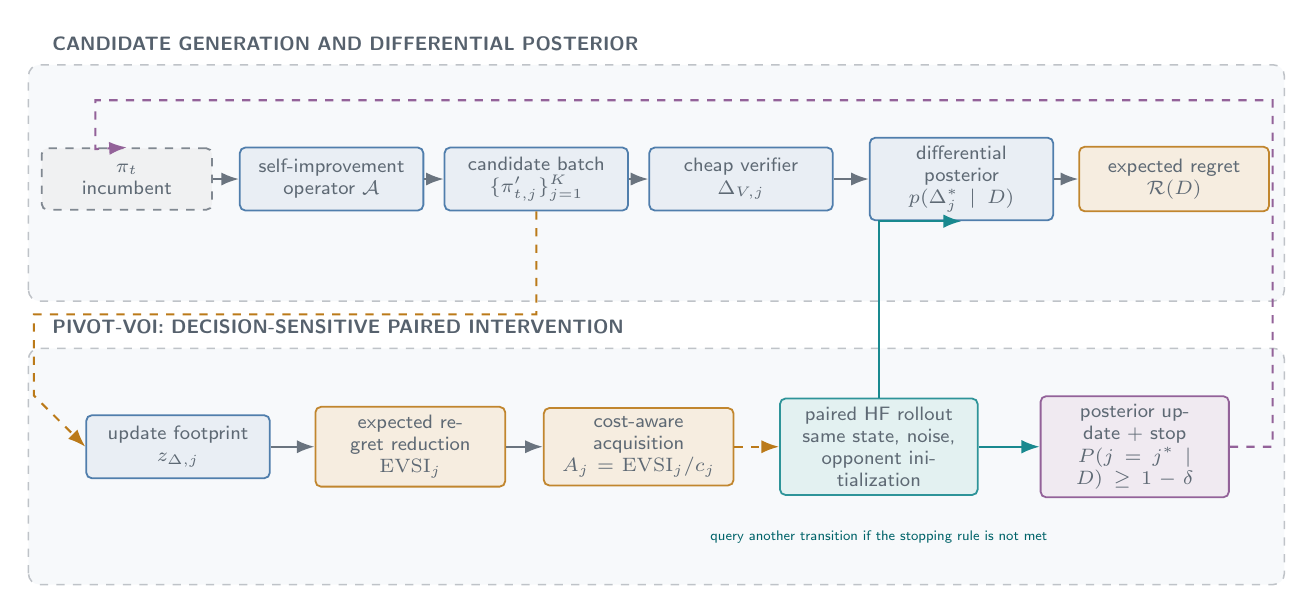
\begin{tikzpicture}[
  x=1cm,y=1cm,>=Latex,
  base/.style={draw=pgray!75,line width=.65pt,rounded corners=2pt,align=center,
    inner sep=3pt,font=\sffamily\scriptsize,text=pgray!95},
  input/.style={base,fill=pgray!9,dashed,text width=1.95cm,minimum height=.78cm},
  process/.style={base,fill=pblue!10,draw=pblue!78,text width=2.12cm,minimum height=.80cm},
  query/.style={base,fill=porange!12,draw=porange!82,text width=2.20cm,minimum height=.82cm},
  hf/.style={base,fill=pteal!11,draw=pteal!82,text width=2.30cm,minimum height=.84cm},
  promote/.style={base,fill=ppurple!11,draw=ppurple!82,text width=2.18cm,minimum height=.82cm},
  arrow/.style={->,draw=pgray!88,line width=.75pt},
  queryarrow/.style={->,draw=porange!90,line width=.75pt,dashed},
  hfarrow/.style={->,draw=pteal!90,line width=.80pt},
  loop/.style={->,draw=ppurple!82,line width=.75pt,dashed},
  band/.style={draw=pgray!38,dashed,rounded corners=4pt,fill=plight,line width=.55pt}
]

% The main figure contains only the decision-critical path.  World-layer
% taxonomy and reporting definitions are documented in the appendix.
\begin{scope}[on background layer]
  \path[band] (.20,2.55) rectangle (16.15,5.55);
  \path[band] (.20,-1.05) rectangle (16.15,1.95);
\end{scope}
\node[font=\sffamily\scriptsize\bfseries,text=pgray,anchor=south west] at (.38,5.61)
  {CANDIDATE GENERATION AND DIFFERENTIAL POSTERIOR};
\node[font=\sffamily\scriptsize\bfseries,text=pgray,anchor=south west] at (.38,2.01)
  {PIVOT-VOI: DECISION-SENSITIVE PAIRED INTERVENTION};

% Stage 1: candidate generation and the cheap signal.
\node[input] (inc) at (1.45,4.10) {$\pi_t$\\incumbent};
\node[process] (op) at (4.05,4.10) {self-improvement\\operator $\mathcal A$};
\node[process] (batch) at (6.65,4.10) {candidate batch\\$\{\pi'_{t,j}\}_{j=1}^{K}$};
\node[process] (proxy) at (9.25,4.10) {cheap verifier\\$\Delta_{V,j}$};
\node[process] (posterior) at (12.05,4.10) {differential posterior\\$p(\Delta^*_j\mid D)$};
\node[query] (regret) at (14.75,4.10) {expected regret\\$\mathcal R(D)$};
\draw[arrow] (inc) -- (op);
\draw[arrow] (op) -- (batch);
\draw[arrow] (batch) -- (proxy);
\draw[arrow] (proxy) -- (posterior);
\draw[arrow] (posterior) -- (regret);

% Stage 2: footprint-aware, cost-aware acquisition and paired evidence.
\node[process] (foot) at (2.10,.70) {update footprint\\$z_{\Delta,j}$};
\node[query] (evsi) at (5.05,.70) {expected regret reduction\\$\mathrm{EVSI}_j$};
\node[query] (cost) at (7.95,.70) {cost-aware acquisition\\$A_j=\mathrm{EVSI}_j/c_j$};
\node[hf] (paired) at (11.00,.70) {paired HF rollout\\same state, noise,\\opponent initialization};
\node[promote] (stop) at (14.25,.70) {posterior update + stop\\$P(j=j^*\mid D)\ge1-\delta$};
% Route the footprint signal through the clear left-side channel between bands;
% it never crosses the section label or another node.
\draw[queryarrow] (batch.south) -- (6.65,2.38) -- (.27,2.38) -- (.27,1.35) -- (foot.west);
\draw[arrow] (foot) -- (evsi);
\draw[arrow] (evsi) -- (cost);
\draw[queryarrow] (cost) -- (paired);
\draw[hfarrow] (paired) -- (stop);
\draw[hfarrow] (paired.north) |- (posterior.south);
\draw[loop] (stop.east) -- (16.00,.70) -- (16.00,5.10) -- (1.05,5.10) -- (1.05,4.48) -- (inc.north);
\node[font=\sffamily\tiny,text=pteal!80!black,align=center] at (11.00,-.45)
  {query another transition if the stopping rule is not met};
\end{tikzpicture}
\end{document}
